\documentclass{article}
\usepackage{graphicx}
\usepackage{lipsum} % For generating placeholder text
\usepackage{subcaption}
\usepackage{dirtree} 
\title{Dating Website Report}
\author{Shyam Sri Vardhan Varri}
\date{\today}

\begin{document}

\maketitle

\section{Introduction}
 This report outlines the design and functionality of a dating website aimed at helping users find their perfect match.

\section{Requirements}

\subsection{Languages}
The development of the dating website will require proficiency in the following languages and technologies:

\begin{itemize}
    \item \textbf{HTML/CSS}: For building the front-end user interface and styling.
    \item \textbf{JavaScript}: For implementing client-side interactivity and dynamic features.
    \item \textbf{Node.js}: For building the back-end server and handling server-side logic.
    \item \textbf{Express.js}: A Node.js web application framework for routing and middleware.
\end{itemize}   
Note that both the \textbf{EJS} and \textbf{Nodejs} work together.


\section{Functionality}
The dating website will function as follows(includes both the basic task and customisations):

\begin{enumerate}
    \item \textbf{User Registration}: Users will sign up for the website by providing basic information and creating a profile.
    \item \textbf{Profile Creation}: Users will fill out their profiles with details about themselves, such as their interests and hobbies.
    \item \textbf{Matching}: The website's matching algorithm will analyze user profiles and suggest potential matches based on compatibility.
    \item \textbf{Communication}: Matched users will be able to communicate with each other through the website's messaging system.
    \item \textbf{Finding a Perfect Match}: The ultimate goal of the website is to help users find their perfect match and form meaningful connections.
\end{enumerate}

\section{Implementation Details}
The customizations were implemented using Node.js for the server-side logic and EJS (Embedded JavaScript) for server-side templating. The following details highlight key aspects of the implementation:


    \subsection{\textbf{Node.js Integration}}  Node.js was utilized to develop the server-side components of the project. It provided a better runtime environment for executing JavaScript code on the server, allowing for efficient handling of HTTP requests and responses.
  \begin{figure}[htbp] 
    \centering 
    \begin{subfigure}[b]{0.45\textwidth} 
        \centering 
        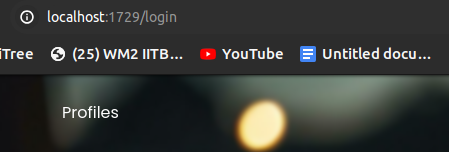
\includegraphics[width=\textwidth]{hosting.png}
        \caption{Local Host} 
        \label{host} 
    \end{subfigure}
    \hfill % Add horizontal space between the subfigures
    \begin{subfigure}[b]{0.45\textwidth} 
        \centering % Center the second image
        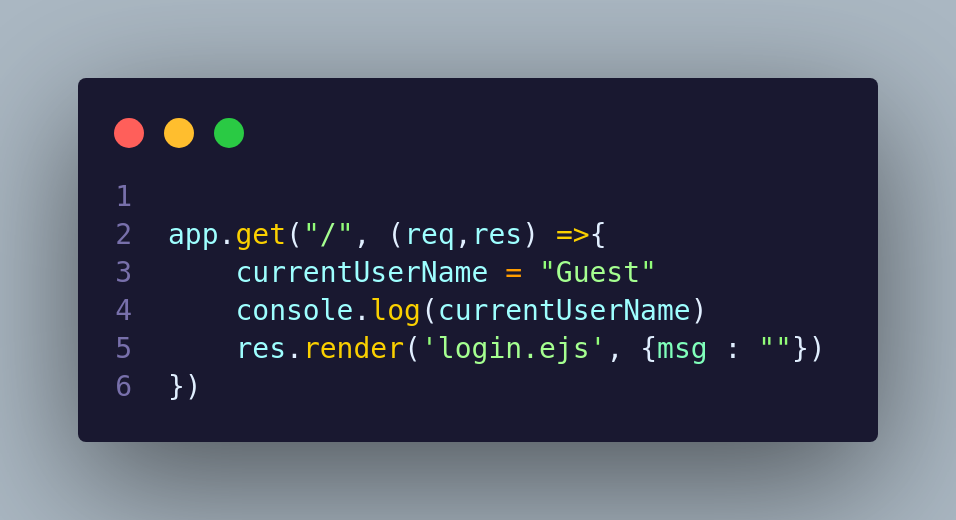
\includegraphics[width=\textwidth]{codenode.png} 
        \caption{Code snippet} % Add a caption to the second image
        \label{node} % Add a label for referencing
    \end{subfigure}
    \caption{} % Add a caption to the entire figure
    \label{NodeJs} % Add a label for referencing
\end{figure}

\subsection{\textbf{EJS Templating}} EJS was employed for server-side templating, enabling dynamic generation of HTML content based on data passed from the server. This facilitated the creation of dynamic web pages with reusable components and layouts.

\begin{figure}[htbp] 
    \centering 
    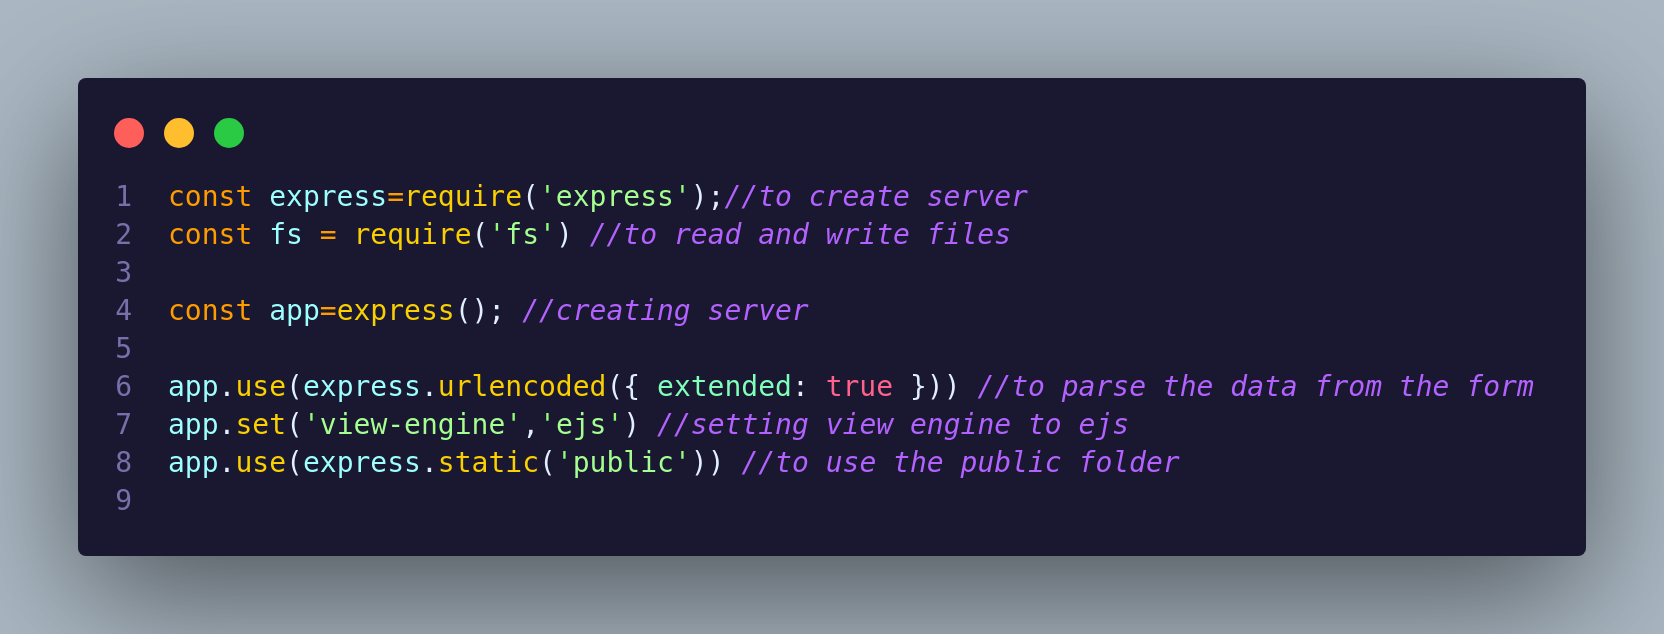
\includegraphics[width=0.5\textwidth]{codeesj.png} 
    \caption{Ejs} 
    \label{Ejs} 
\end{figure}

  \subsection{\textbf{Sorting Functionality}} A custom sorting function was implemented to arrange user profiles based on rating and gender classification. The sorting algorithm arranges profiles in descending order(due to insufficient time, only descending order is embedded), prioritizing profiles with higher ratings and ensuring gender classification alignment as per user preferences.
    
\begin{figure}[htbp] 
    \centering 
    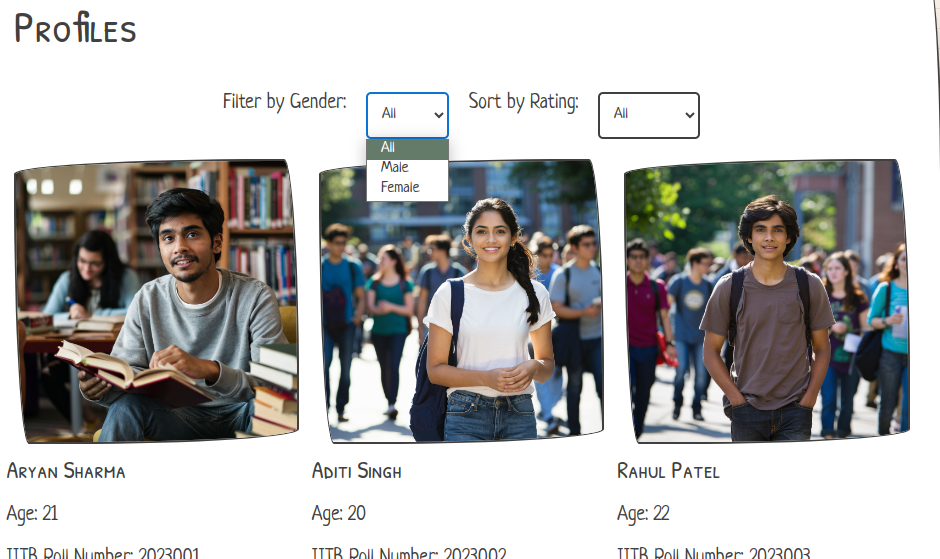
\includegraphics[width=0.5\textwidth]{filter.png} 
    \caption{filter} 
    \label{filter} 
    \end{figure}
\section{User Authentication and Registration}

In this section, we discuss the processes involved in user authentication, forgot password functionality, and user registration for the dating website project.

\subsection{Login Authentication}

The login authentication process ensures that only registered users with valid credentials can access the website. Here's how it works:

\begin{enumerate}
    \item The user navigates to the login page of the website.
    \item The user enters their username and password.
    \item The system validates the user's credentials against the database.
    \item If the credentials are correct, the user is granted access to their account and redirected to their dashboard. Otherwise, an error message is displayed.
\end{enumerate}
\begin{figure}[htbp] 
    \centering 
    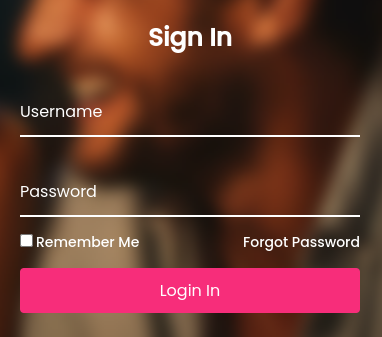
\includegraphics[width=0.5\textwidth]{login.png} 
    \caption{Login} 
    \label{Login} 
    \end{figure}


\subsection{Forgot Password}

The forgot password functionality allows users to reset their passwords if they forget them. Here's the procedure:

\begin{enumerate}
    \item The user clicks on the "Forgot Password" link on the login page.
    \item The system prompts the user to enter their username.
    \item The system retrieves a secret question from the database and sends it to the html page and renders on the page.
    \item The user enters the secret answer of that question.
    \item The system validates the answer and prints the password for the corresponding username.
\end{enumerate}
\begin{figure}[htbp] 
    \centering 
    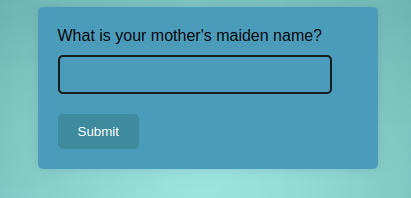
\includegraphics[width=0.5\textwidth]{forgot.png} 
    \caption{Forgot-password} 
    \label{forgot-password} 
    \end{figure}

\subsection{User Registration}

The user registration process allows new users to create accounts on the dating website. Here's how it works:

\begin{enumerate}
    \item The user navigates to the registration page of the website.
    \item The user fills out the registration form, providing details such as their username, password,secret question,secret answer.
    \item The system validates the user's input, ensuring that all required fields are filled and username is unique.
    \item If the validation is successful, the user's account is created, and they are logged in automatically. Otherwise, error messages are displayed to guide the user in correcting their input.
\end{enumerate}

\begin{figure}[htbp] 
    \centering 
    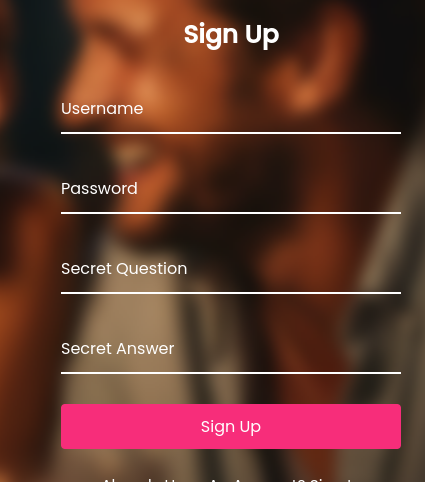
\includegraphics[width=0.5\textwidth]{register.png} 
    \caption{SignUp} 
    \label{SIgnUp} 
    \end{figure}

\section{File Structure}
The following is the file structure of the project folder:

\dirtree{%
.1 / (Root Directory).
.2 server.js.
.2 package.json.
.2 package-lock.json.
.2 node-modules.
.2 views.
.3 dating.ejs.
.3 profiles.ejs.
.3 login.ejs.
.3 forgot.ejs.
.2 public.
.3 css.
.4 style.css.
.4 login.css.
.3 js.
.4 script1.js.
.4 script2.js.
.3 \ldots.
}
\section{File Handling}

To handle files in the project, follow these steps:

\begin{enumerate}
    \item \textbf{Open the Zip File:} First, unzip the provided project file.
    \item \textbf{Navigate to the Project Directory:} Open a terminal window and navigate to the project directory using the \texttt{cd} command.
    \item \textbf{Start the Server:} Run the following command in the terminal to start the server:
    \begin{verbatim}
    npm run devStart
    \end{verbatim}
    This command will start the server, and it will be accessible at \texttt{localhost:1729}.
    \begin{figure}[htbp] 
    \centering 
    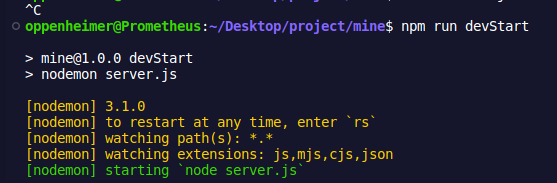
\includegraphics[width=0.5\textwidth]{server.png} 
    \caption{server} 
    \label{server} 
    \end{figure}
    \item \textbf{Replace \texttt{students.json} and \texttt{login.json}:} 
    Locate the \texttt{students.json} and \texttt{login.json} files in the project directory. Replace these files with the real data files you want to use.
    \item \textbf{Update File References:} Check for all locations where the \texttt{login.json} and \texttt{students.json} files are used in your project. Update these references to point to the new files you replaced in the previous step.
\end{enumerate}

Make sure to save all changes and restart the server (this will be automatically done as we are using an extra extension devStart).\\
Now you can login and explore the website!!


\end{document}
